\hypertarget{index_runStandAloneMode}{}\section{Running C\+L\+A\+S\+S-\/\+C\+T\+E\+M}\label{index_runStandAloneMode}
\href{https://docs.google.com/document/d/1pzp7UfNe6aVFXe9LI9XMiGUX2pCALk4tU8MqF_UpQLg/edit?usp=sharing}{\tt Guide to running C\+L\+A\+S\+S-\/\+C\+T\+E\+M in a stand-\/alone mode}\hypertarget{index_overviewCTEM}{}\section{Overview of C\+T\+E\+M}\label{index_overviewCTEM}
Version 1 of the C\+T\+E\+M is the terrestrial carbon cycle component of the second generation Canadian Earth System Model (Can\+E\+S\+M2) \cite{Arora2011-79f} where it is coupled to version 2.\+7 of the Canadian Land Surface Scheme (C\+L\+A\+S\+S). C\+T\+E\+M v. 2.\+0, used here, is currently coupled to the C\+L\+A\+S\+S v. 3.\+6 \cite{Verseghy2012-c0e}. The coupled C\+L\+A\+S\+S--C\+T\+E\+M model is capable of being run online in the Can\+E\+S\+M model or offline, as is the case in this study, driven by observation-\/based meteorological forcings. C\+T\+E\+M models terrestrial ecosystem processes for nine P\+F\+Ts, two of which are crop P\+F\+Ts (see Table tab\+:compparams\}), by tracking the flow of carbon through three living vegetation components (leaves, stem and roots) and two dead carbon pools (litter and soil). The carbon budget equations for the model\textquotesingle{}s five pools are summarized in Sect. rate\+\_\+change\+\_\+eqns\} of the Appendix. The amount of carbon in these five carbon pools is simulated prognostically. C\+L\+A\+S\+S models the land surface energy and water balance and calculates liquid and frozen soil moisture, and soil temperature for three soil layers (with thicknesses 0.\+1, 0.\+25 and 3.\+75\textbackslash{}, $m$). In the C\+L\+A\+S\+S--C\+T\+E\+M framework, C\+L\+A\+S\+S uses structural vegetation attributes (including L\+A\+I, vegetation height, canopy mass and rooting depth) simulated by C\+T\+E\+M, and C\+T\+E\+M uses soil moisture, soil temperature and net radiation calculated by C\+L\+A\+S\+S. Combined, C\+L\+A\+S\+S and C\+T\+E\+M simulate the atmosphere--land fluxes of energy, water and $CO_2$.

Version 1.\+0 of C\+T\+E\+M is described in a collection of papers detailing parametrization of photosynthesis, autotrophic and heterotrophic respiration \cite{Arora2003-3b7}; phenology, carbon allocation, biomass turnover and conversion of biomass to structural attributes \cite{Arora2005-6b1}; dynamic root distribution \cite{Arora2003838}; and disturbance (fire) \cite{Arora20052ac}. These processes are modelled over prescribed fractional coverage of nine P\+F\+Ts \cite{Wang2006-he} and determine the structural vegetation dynamics including vegetation biomass, L\+A\+I, vegetation height, fraction of roots in each of the three soil layers, leaf onset and offset times and primary $CO_2$ fluxes of gross primary productivity (G\+P\+P) and N\+P\+P. A full description of C\+T\+E\+M and changes from v. 1.\+0 to v. 2.\+0 are included in the Appendix.

A parametrization for competition between P\+F\+Ts in an earlier version of C\+T\+E\+M is described by \cite{Arora2006-pp} \cite{Arora2006-ax} where it was evaluated at select locations. Here we present C\+T\+E\+M v. 2.\+0, which builds upon the model framework of C\+T\+E\+M v. 1.\+0 and can be run in two different modes, either (i) using specified fractional coverage of its nine P\+F\+Ts, or (ii) allowing the fractional coverage of its seven non-\/crop P\+F\+Ts to be dynamically determined based on competition between P\+F\+Ts. The parametrization for simulating competition between P\+F\+Ts is summarized in Sect. compmain\}. The fire parametrization has also been refined in the new model version as described in Appendix fire\}. The C\+L\+A\+S\+S--C\+T\+E\+M modelling framework has the capability of representing the sub-\/grid scale variability of P\+F\+Ts using either a composite or a mosaic configuration \cite{Li2012-f7f} \cite{Melton2014-xk}. In the composite (or single tile) configuration, the vegetation attributes for all P\+F\+Ts present in a grid cell are averaged and used in energy and water balance calculations that determine the physical land surface conditions including soil moisture, soil temperature and thickness and fractional coverage of snow (if present). In the mosaic (or multi-\/tile) configuration each P\+F\+T is allocated its own tile for which separate energy and water balance calculations are performed. As a result, the simulated carbon balance evolves somewhat differently in the two configurations despite being driven with identical climate forcing (see \cite{Melton2014-xk}). The results presented in this paper are obtained using the composite configuration.\hypertarget{index_overviewCLASS}{}\section{Overview of C\+L\+A\+S\+S}\label{index_overviewCLASS}
The Canadian Land Surface Scheme, C\+L\+A\+S\+S, was originally developed for use with the Canadian Global Climate Model or G\+C\+M (Verseghy, 1991; Verseghy et al., 1993). This documentation describes version 3.\+6 of C\+L\+A\+S\+S, which was released in December of 2011. The table at the end of this overview summarizes the development of C\+L\+A\+S\+S from the late 1980’s to the present.

The basic function of C\+L\+A\+S\+S is to integrate the energy and water balances of the land surface forward in time from an initial starting point, making use of atmospheric forcing data to drive the simulation. When C\+L\+A\+S\+S is run in coupled mode with a global or regional atmospheric model, the required forcing data are passed to it at each time step over each modeled grid cell from the atmospheric driver. C\+L\+A\+S\+S then performs its internal calculations, evaluating a suite of prognostic and diagnostic variables such as albedo and surface radiative and turbulent fluxes, which are in turn passed back to the driver. C\+L\+A\+S\+S can also be run in uncoupled or offline mode, using forcing data derived from field measurements, and the output values of its prognostic and diagnostic variables can then be validated against observations. Version 3.\+6 includes a single-\/column offline driver which can be used for this purpose.

C\+L\+A\+S\+S models separately the energy and water balances of the soil, snow, and vegetation canopy (see the diagram below). The basic prognostic variables consist of the temperatures and the liquid and frozen moisture contents of the soil layers; the mass, temperature, density, albedo and liquid water content of the snow pack; the temperature of the vegetation canopy and the mass of intercepted rain and snow present on it; the temperature and depth of ponded water on the soil surface; and an empirical vegetation growth index. These variables must be initialized, and a set of physical parameters describing the soil and vegetation existing on the modelled area must be assigned background values, at the beginning of the simulation.

At each time step, C\+L\+A\+S\+S calculates the bulk characteristics of the vegetation canopy on the basis of the vegetation types present over the modelled area. In a pre-\/processing step, each vegetation type is assigned representative values of parameters such as albedo, roughness length, annual maximum and minimum plant area index, rooting depth and so on (see the section on “\+Data Requirements”). These values are then aggregated over four main vegetation categories identified by C\+L\+A\+S\+S\+: needleleaf trees, broadleaf trees, crops, and grass (i.\+e. short vegetation). The physiological characteristics of the vegetation in each category are determined at the current time step using the aggregated background parameters and assumed annual or diurnal variation functions. These physiological characteristics are then aggregated to produce the bulk canopy characteristics for the current time step.


\begin{DoxyImage}
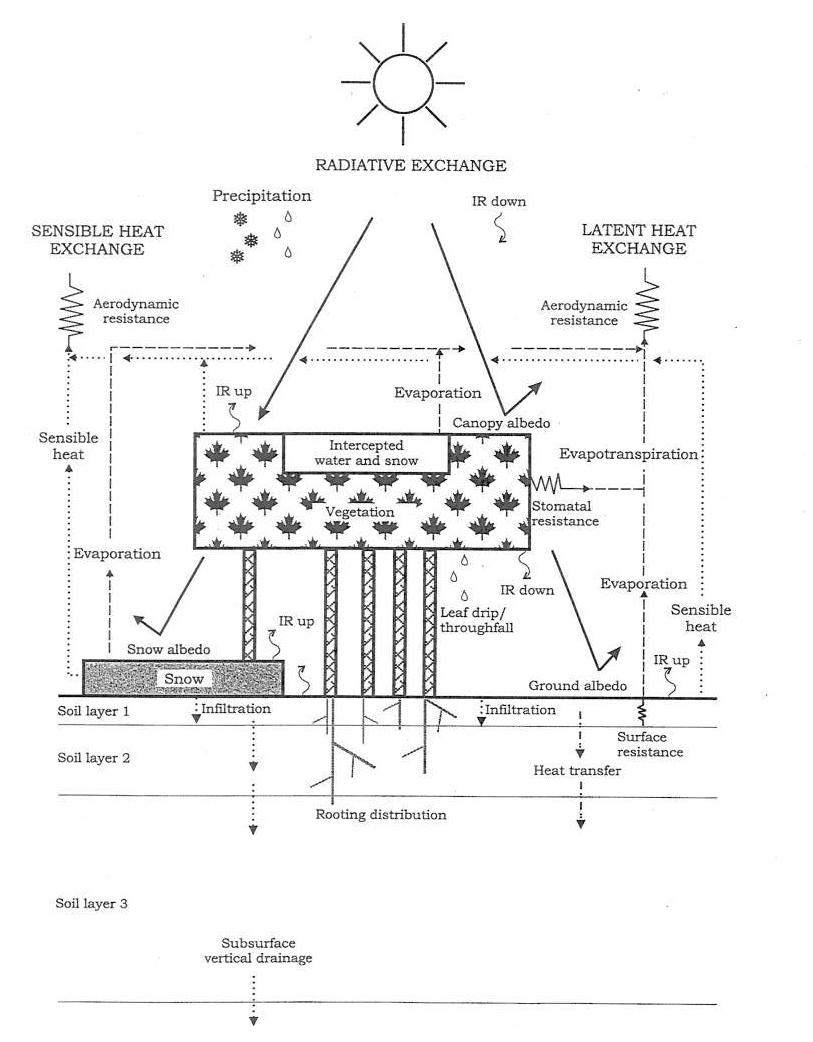
\includegraphics[width=\textwidth,height=\textheight/2,keepaspectratio=true]{schematicDiagramOfClass.png}
\caption{Schematic Diagram Of C\+L\+A\+S\+S}
\end{DoxyImage}
 In performing the surface flux calculations the modeled area is divided into up to four subareas\+: bare soil, vegetation over soil, snow over bare soil, and vegetation over snow. The fractional snow coverage is determined using the concept of a threshold snow depth. If the calculated snow depth is less than this value, the snow depth is set to the threshold value and the fractional snow cover is calculated on the basis of conservation of snow mass. The fluxes are calculated for each of the four subareas, and these and the prognostic variables are then areally averaged before being passed back to the atmospheric model.

Originally C\+L\+A\+S\+S performed only one set of these calculations for each grid cell of the model domain. In more recent versions, a “mosaic” option has been added to handle sub-\/grid scale heterogeneity more effectively. When this option is utilized, each grid cell is divided into a user-\/specified number of mosaic “tiles”, and the C\+L\+A\+S\+S calculations are performed in turn over each. The surface fluxes are averaged, but the prognostic variables are kept separate for each of the tiles of the mosaic between time steps.

The section on the C\+L\+A\+S\+S offline driver, R\+U\+N\+C\+L\+A\+S\+S, provides information on how a C\+L\+A\+S\+S run is typically performed, from assigning the background and initial values of variables, through calling the high-\/level C\+L\+A\+S\+S subroutines, to calculating values of diagnostic and output variables. A gather-\/scatter operation is included in the driver, mimicking the practice in atmospheric models of “gathering” land surface points on latitude circles onto long vectors prior to the calculations, for improved computational efficiency on vector supercomputers. For C\+L\+A\+S\+S, the mosaic tiles on each of the modelled grid cells are “gathered” onto long arrays prior to calling the C\+L\+A\+S\+S subroutines (thus collapsing the first two dimensions of the arrays into one), and subsequently “scattered” back onto the grid cells before performing the diagnostic averaging calculations.

The two sections following the one that describes the driver provide detailed descriptions first of the common block and other preliminary routines that are called before the run is launched, and then of the pre-\/ and post-\/processing routines that are called at the beginning and end of each time step. The next three sections detail the three main C\+L\+A\+S\+S subroutines together with the auxiliary subroutines that they call\+: C\+L\+A\+S\+S\+A, which handles the calculation of the albedos and other surface parameters; C\+L\+A\+S\+S\+T, which addresses the evaluation of the surface energy balance and related variables; and C\+L\+A\+S\+S\+W, which performs the surface water balance calculations and the re-\/aggregation of the prognostic variables. The sub-\/section on each subroutine contains a dictionary of the variables passed into and out of it, with units. The final section provides a list of references cited.\hypertarget{index_devHistory}{}\section{Developmental history of C\+L\+A\+S\+S}\label{index_devHistory}
\[ \begin{tabular}{ | l | l || l | } 1.0 & April 1989 & Basic thermal and hydrological model of snow and soil. \\ 2.0 & August 1991 & Addition of vegetation thermal and hydrological model. \\ 2.1 & May 1993 & Full vectorization of code to enable efficienr running on vector supercomputers. \\ 2.2 & April 1994 & Augmentation of diagnostic calculations; incorporation of in-line comments throughout; development of a parallel stand-alone version of the model for use with field data. \\ 2.3 & December 1994 & Revisions to diagnostic calculations; new near-surface atmospheric stability functions. \\ 2.4 & August 1995 & Complete set of water budget diagnostic calculations; parametrizations of organic soils and rock soils; allowance for inhomegeneity between soil layers; incorporation of variable surface detention capacity. \\ 2.5 & January 1996 & Completion of energy budget diagnostic calculations. \\ 2.6 & August 1997 & Revisions to surface stability function calculations. \\ 2.7 & December 1997 & Incorporation of variable soil permeable depth; calculation of soil thermal and hydraulic properties based on textural composition; modified surface temperature iteration scheme. \\ 3.0 & December 2002 & Improved treatment of soil evaporation; complete treatment of organic soils; new canopy conductance formulation; preliminary routines for lateral movement of soil water; enhanced snow density and snow interception; improved turbulent transfer from vegetation; mosaic formulation. \\ 3.1 & April 2005 & Faster surface temperature iteration scheme; refinements to leaf boundary resistance formulation; improved treatment of snow sublimation and interception; transition to Fortran 90 and single precision variables. \\ 3.2 & May 2006 & Option for multiple soil layers at depth; additional liquid water content of snow pack; revised radiation transmission in vegetation. \\ 3.3 & December 2006 & Separate temperature profile curve fit for snow and soil; multiple-layer option for ice sheets; water and energy balance checks for each time step; modifications to soil hydraulic conductivity calculations. \\ 3.4 & April 2008 & Streamline and clean up code; updated soil thermal conductivity calculations; revisions to handling of water stored on vegetation. \\ 3.5 & December 2010 & Updated field capacity calculation; revised treatment of water on canopy; reworked calculation of baseflow. \\ 3.6 & December 2011 & Revised ponding depth over organic soils; revised snow albedo refreshment threshold; new snow thermal conductivity algorithm; interface with Canadian Terrestrial Ecosystem Model (CTEM). \\ \end{tabular} \]\hypertarget{index_dataRequirements}{}\section{Data Requirements}\label{index_dataRequirements}
This section describes the three types of data that are required to run C\+L\+A\+S\+S\+: atmospheric forcing data, surface vegetation and soil data, and initial values for the prognostic variables.\hypertarget{index_forcingData}{}\subsection{Forcing Data}\label{index_forcingData}
At each time step, for each grid cell or modelled area, the following atmospheric forcing data are required\+:


\begin{DoxyItemize}
\item F\+C\+L\+O\+R\+O\+W Fractional cloud cover \mbox{[} \mbox{]}
\item F\+D\+L\+R\+O\+W Downwelling longwave sky radiation $[ W m^{-2} ]$
\item F\+S\+I\+H\+R\+O\+W Near infrared shortwave radiation incident on a horizontal surface $[W m^{-2} ]$
\item F\+S\+V\+H\+R\+O\+W Visible shortwave radiation incident on a horizontal surface $[W m^{-2} ]$
\item P\+R\+E\+R\+O\+W Surface precipitation rate $[kg m^{-2} s^{-1} ]$
\item P\+R\+E\+S\+R\+O\+W Surface air pressure $[P_a ]$
\item Q\+A\+R\+O\+W Specific humidity at reference height $[kg kg^{-1} ]$
\item T\+A\+R\+O\+W Air temperature at reference height \mbox{[}K\mbox{]}
\item U\+L\+R\+O\+W Zonal component of wind velocity $[m s^{-1} ]$
\item V\+L\+R\+O\+W Meridional component of wind velocity $[m s^{-1} ]$
\item V\+M\+O\+D\+R\+O\+W Wind speed at reference height $[m s^-1 ]$
\item Z\+B\+L\+D\+R\+O\+W Atmospheric blending height for surface roughness length averaging \mbox{[}m\mbox{]}
\item Z\+R\+F\+H\+R\+O\+W Reference height associated with forcing air temperature and humidity \mbox{[}m\mbox{]}
\item Z\+R\+F\+M\+R\+O\+W Reference height associated with forcing wind speed \mbox{[}m\mbox{]}
\end{DoxyItemize}

When assembling the forcing data, the following guidelines should be noted\+:

1) C\+L\+A\+S\+S ordinarily requires that the forcing incoming shortwave radiation be partitioned into the visible and near-\/infrared components. If these are not available, however, they can each be roughly estimated as approximately half of the total incoming solar radiation.

2) The fractional cloud cover is used to calculate the direct and diffuse components of the incoming shortwave radiation. If it is not available it can be estimated on the basis of the solar zenith angle and the occurrence of precipitation (see the section on the R\+U\+N\+C\+L\+A\+S\+S driver).

3) For atmospheric models, the air temperature supplied to C\+L\+A\+S\+S should be the lowest level air temperature extrapolated using the dry adiabatic lapse rate to the bottom of the atmosphere, i.\+e. to where the wind speed is zero and the pressure is equal to the surface pressure P a . For field data, the actual measured air temperature at the reference height should be used, since in this case the adiabatic extrapolation is performed within C\+L\+A\+S\+S.

4) Atmospheric models provide the zonal and meridional components of the wind velocity, but C\+L\+A\+S\+S does not actually require information on wind direction. Thus, if only the scalar wind speed is available, either U\+L\+R\+O\+W or V\+L\+R\+O\+W can be set to it, and the other to zero. (Both of these terms, plus the scalar wind speed V\+M\+O\+D\+R\+O\+W, must be supplied to C\+L\+A\+S\+S.)

5) In atmospheric models the forcing wind speed, air temperature and specific humidity are obtained from the lowest modelled atmospheric layer, and thus the reference height will be the height above the “surface” (i.\+e. the location where the wind speed is zero and the pressure is equal to the surface pressure P a ) corresponding to that lowest layer. Some atmospheric models use a vertical co-\/ordinate system in which the momentum and thermodynamic levels are staggered, and if so, Z\+F\+R\+M\+R\+O\+W and Z\+R\+F\+H\+R\+O\+W will have different values. If that is the case, the switch I\+S\+L\+F\+D in the C\+L\+A\+S\+S driver should be set to 2, so that the subroutines F\+L\+X\+S\+U\+R\+F\+Z and D\+I\+A\+S\+U\+R\+F\+Z are called (see the R\+U\+N\+C\+L\+A\+S\+S documentation), since the other options do not support different reference heights. In the case of field data, the reference height is the height above the ground surface at which the variables are measured. If the measurement height for wind speed is different from that for the air temperature and specific humidity, again the I\+S\+L\+F\+D switch in the C\+L\+A\+S\+S driver should be set to 2. (Note that neither Z\+R\+F\+H\+R\+O\+W nor Z\+R\+F\+M\+R\+O\+W may be smaller than the vegetation canopy height, as this will cause the model run to crash.)

6) If the surface being modelled is a heterogeneous one, care must be taken to ensure that the reference heights are greater than the “blending height”, the distance above the surface at which the atmospheric variables are not dominated by any one surface type. In principle this height depends on the length scale of the roughness elements; it is usually of the order of 50-\/100 m. In C\+L\+A\+S\+S the blending height is used in averaging the roughness lengths over the modelled area, and is read in separately from Z\+R\+F\+M\+R\+O\+W and Z\+R\+F\+H\+R\+O\+W as Z\+B\+L\+D\+R\+O\+W.

7) C\+L\+A\+S\+S is able to run with total incoming precipitation, partitioning it into rainfall and snowfall on the basis of empirically derived equations. If the rainfall rate (R\+P\+R\+E\+R\+O\+W) and snowfall rate (S\+P\+R\+E\+R\+O\+W) are available, they should be used instead. The R\+E\+A\+D statement in the C\+L\+A\+S\+S driver should be modified accordingly, and the switch I\+P\+C\+P should be set to 4.

8) The length of the time step should be carefully considered in assembling the forcing data. C\+L\+A\+S\+S has been designed to run at a time step of 30 minutes or less, and the explicit prognostic time stepping scheme used for the soil, snow and vegetation variables is based on this assumption. Longer time steps may lead to the appearance of numerical instabilities in the modelled prognostic variables.\hypertarget{index_vegetationData}{}\subsection{Vegetation Data}\label{index_vegetationData}
For each of the four main vegetation categories (needleleaf trees, broadleaf trees, crops and grass), the following data are required for each mosaic tile over each grid cell or modelled area\+:


\begin{DoxyItemize}
\item A\+L\+I\+C\+R\+O\+T Average near-\/\+I\+R albedo of vegetation category when fully-\/leafed \mbox{[} \mbox{]}
\item A\+L\+V\+C\+R\+O\+T Average visible albedo of vegetation category when fully-\/leafed \mbox{[} \mbox{]}
\item C\+M\+A\+S\+R\+O\+T Annual maximum canopy mass for vegetation category $[kg m^{-2} ]$
\item F\+C\+A\+N\+R\+O\+T Annual maximum fractional coverage of modelled area \mbox{[} \mbox{]}
\item L\+N\+Z0\+R\+O\+T Natural logarithm of maximum vegetation roughness length \mbox{[} \mbox{]}
\item P\+A\+M\+N\+R\+O\+T Annual minimum plant area index of vegetation category \mbox{[} \mbox{]}
\item P\+A\+M\+X\+R\+O\+T Annual maximum plant area index of vegetation category \mbox{[} \mbox{]}
\item P\+S\+G\+A\+R\+O\+T Soil moisture suction coefficient (used in stomatal resistance calculation) \mbox{[} \mbox{]}
\item P\+S\+G\+B\+R\+O\+T Soil moisture suction coefficient (used in stomatal resistance calculation) \mbox{[} \mbox{]}
\item Q\+A50\+R\+O\+T Reference value of incoming shortwave radiation (used in stomatal resistance calculation) $[W m^{-2} ]$
\item R\+O\+O\+T\+R\+O\+T Annual maximum rooting depth of vegetation category \mbox{[}m\mbox{]}
\item R\+S\+M\+N\+R\+O\+T Minimum stomatal resistance of vegetation category $[s m^{-1} ]$
\item V\+P\+D\+A\+R\+O\+T Vapour pressure deficit coefficient (used in stomatal resistance calculation) \mbox{[} \mbox{]}
\item V\+P\+D\+B\+R\+O\+T Vapour pressure deficit coefficient (used in stomatal resistance calculation) \mbox{[} \mbox{]}
\end{DoxyItemize}

C\+L\+A\+S\+S models the physiological characteristics of trees as remaining constant throughout the year except for the leaf area index and plant area index, which vary seasonally between the limits defined by P\+A\+M\+X\+R\+O\+T and P\+A\+M\+N\+R\+O\+T. The areal coverage of crops varies from zero in the winter to F\+C\+A\+N\+R\+O\+T at the height of the growing season, and their physiological characteristics undergo a corresponding cycle. Grasses remain constant year-\/round. (For full details of these calculations, see the documentation for subroutine A\+P\+R\+E\+P). Urban areas are also treated as “vegetation” in the C\+L\+A\+S\+S code, and have associated values for F\+C\+A\+N\+R\+O\+T, A\+L\+V\+C\+R\+O\+T, A\+L\+I\+C\+R\+O\+T and L\+N\+Z0\+R\+O\+T. Thus these arrays have a third dimension of 5 rather than 4.

Ideally the above vegetation parameters should be measured at the modelled location. Of course this is not always possible, especially when running over a large modelling domain. As a guide, the table in Appendix A provides representative values for the 20 vegetation types recognized by the Canadian G\+C\+M. If more than one type of vegetation in a given category is present on the modelled area, the parameters for the category should be areally averaged over the vegetation types present. For the stomatal resistance parameters, typical values of these for the four principal vegetation types are given below\+:

\[ \begin{tabular}{ | l | l | l | l | l | l | l | } & RSMN & QA50 & VPDA & VPDB & PSGA & PSGB \\ Needleleaf trees & 200.0 & 30.0 & 0.65 & 1.05 & 100.0 & 5.0 \\ Broadleaf trees & 125.0 & 40.0 & 0.50 & 0.60 & 100.0 & 5.0 \\ Crops & 85.0 & 30.0 & 0.50 & 1.00 & 100.0 & 5.0 \\ Grass & 100.0 & 30.0 & 0.50 & 1.00 & 100.0 & 5.0 \\ \end{tabular} \]\hypertarget{index_soilData}{}\subsection{Soil Data}\label{index_soilData}
The following information is required for each modelled soil layer\+:


\begin{DoxyItemize}
\item D\+E\+L\+Z Layer thickness \mbox{[}m\mbox{]}
\item Z\+B\+O\+T Depth of bottom \mbox{[}m\mbox{]}
\end{DoxyItemize}

The standard operational configuration for C\+L\+A\+S\+S consists of three soil layers, of thicknesses 0.\+10 m, 0.\+25 m and 3.\+75 m, and thus of bottom depths 0.\+10, 0.\+35 and 4.\+10 m respectively. C\+L\+A\+S\+S versions 3.\+2 and higher support other options\+: the third soil layer may be replaced with a larger number of thinner layers, and/or the bottom of the soil profile may be extended below 4.\+10 m. However, because the temperature stepping scheme used in C\+L\+A\+S\+S is of an explicit formulation, care must be taken not to make the layers too thin, since this may lead to numerical instability problems. As a rule of thumb, the thicknesses of layers deeper than the first should be limited to $\geq$ 0.\+25 m.

For each of the modelled soil layers on each of the mosaic tiles, the following texture data are required\+:


\begin{DoxyItemize}
\item C\+L\+A\+Y\+R\+O\+T Percentage clay content
\item O\+R\+G\+M\+R\+O\+T Percentage organic matter content
\item S\+A\+N\+D\+R\+O\+T Percentage sand content
\end{DoxyItemize}


\begin{DoxyImage}
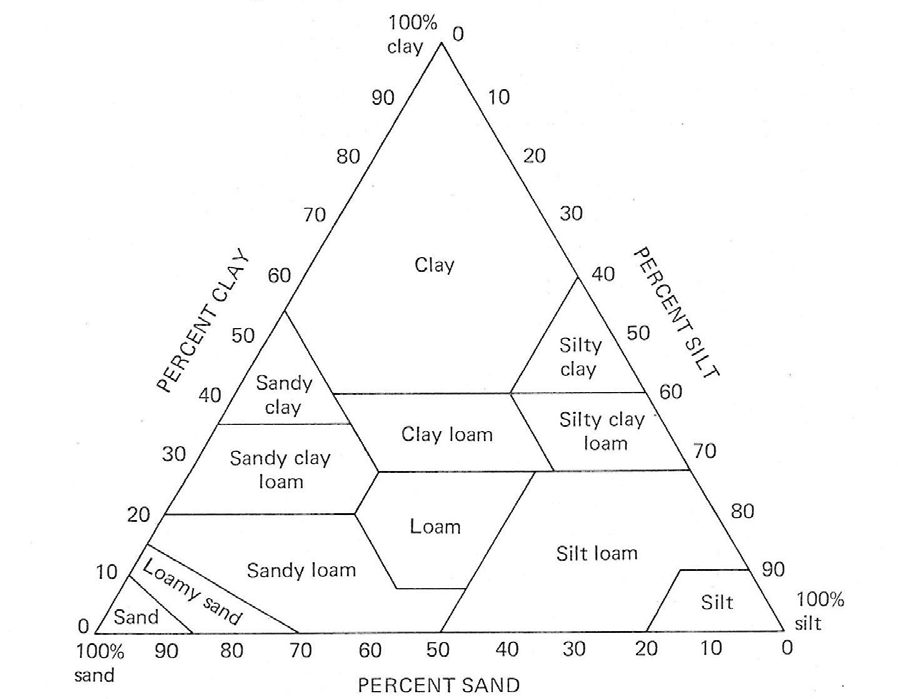
\includegraphics[width=\textwidth,height=\textheight/2,keepaspectratio=true]{percentSand.png}
\caption{Percent Sand}
\end{DoxyImage}
 1) For mineral soils, the percentages of sand, clay and organic matter content need not add up to 100\%, since the residual is assigned to silt content. If the exact sand, clay and organic matter contents are not known, estimates can be made for the general soil type on the basis of the standard U\+S\+D\+A texture triangle shown above. Organic matter contents in mineral soils are typically not more than a few percent.

2) If the soil layer is a fully organic one, S\+A\+N\+D\+R\+O\+T, C\+L\+A\+Y\+R\+O\+T and O\+R\+G\+M\+R\+O\+T are used differently. The sand content is assigned a flag value of -\/2, and the organic matter content may be assigned a flag value of 1, 2 or 3 depending on whether the peat texture is fibric, hemic or sapric (see Letts et al., 2000). The current default is for the first layer to be assumed as fibric, the second as hemic and any lower layers as sapric. C\+L\+A\+Y\+R\+O\+T is not used and is set to zero.

3) If the layer consists of rock, S\+A\+N\+D\+R\+O\+T is assigned a flag value of -\/3. If it is part of a continental ice sheet, it is assigned a flag value of -\/4. In both cases, C\+L\+A\+Y\+R\+O\+T and O\+R\+G\+M\+R\+O\+T are not used and are set to zero.

S\+A\+N\+D\+R\+O\+T, C\+L\+A\+Y\+R\+O\+T and O\+R\+G\+M\+R\+O\+T are utilized in the calculation of the soil layer thermal and hydraulic properties in subroutine C\+L\+A\+S\+S\+B. If the measured values of these properties are available, they should be used instead.

For each of the mosaic tiles over the modelled area, the following surface parameters must be specified\+:


\begin{DoxyItemize}
\item D\+R\+N\+R\+O\+T Soil drainage index
\item F\+A\+R\+E\+R\+O\+T Fractional coverage of mosaic tile on the modelled area
\item M\+I\+D\+R\+O\+T Mosaic tile type identifier (1 for land surface, 0 for inland lake)
\item S\+D\+E\+P\+R\+O\+T Soil permeable depth \mbox{[}m\mbox{]}
\end{DoxyItemize}

1) The soil permeable depth, i.\+e. the depth to bedrock, may be less than the modelled thermal depth of the soil profile. This permeable depth is indicated by the variable S\+D\+E\+P\+R\+O\+T. If the depth to bedrock occurs within a soil layer rather than at the interface between two layers, C\+L\+A\+S\+S assigns the specified mineral or organic soil characteristics to the part of the layer above bedrock, and values corresponding to rock to the portion below.

2) The drainage index, D\+R\+N\+R\+O\+T, is set to 1 except in cases of deep soils where it is desired to suppress drainage from the bottom of the soil profile (e.\+g. in bogs, or in deep soils with a high water table). In this case it is set to 0.

When the standard three-\/layer soil configuration is used, C\+L\+A\+S\+S provides a means of accounting for the possibility of the depth to bedrock falling within the thick third layer, and therefore of phase changes of water taking place in only the upper part of the layer, by introducing the variable T\+B\+A\+S\+R\+O\+T, which refers to the temperature of the lower part of the layer containing the bedrock. At the beginning of the time step the temperature of the upper part of the layer is disaggregated from the overall average layer temperature using the saved value of T\+B\+A\+S\+R\+O\+T. The heat flow between the upper part of the soil layer and the lower part is diagnosed from the heat flux at the top of the layer. The upper layer temperature and T\+B\+A\+S\+R\+O\+T are stepped ahead separately, and the net heat flux in the upper part of the layer is used in the phase change of water if appropriate. The upper layer temperature and T\+B\+A\+S\+R\+O\+T are re-\/aggregated at the end of the time step to yield once again the overall average layer temperature.

Two variables, assumed to be constant over the grid cell, are provided if required for atmospheric model runs\+:


\begin{DoxyItemize}
\item G\+G\+E\+O\+R\+O\+W Geothermal heat flux $[W m^{-2} ]$
\item Z0\+O\+R\+R\+O\+W Orographic roughness length \mbox{[}m\mbox{]}
\end{DoxyItemize}

Unless the soil depth is very large and/or the run is very long, the geothermal heat flux can be set to zero. Z0\+O\+R\+R\+O\+W is the surface roughness length representing the contribution of orography or other terrain effects to the overall roughness, which becomes important when the modelled grid cell is very large (e.\+g. in a G\+C\+M). For field studies it can be set to zero.

Finally, four parameters are required for modelling lateral movement of soil water\+: G\+R\+K\+F\+R\+O\+T, W\+F\+C\+I\+R\+O\+T, W\+F\+S\+F\+R\+O\+T and X\+S\+L\+P\+R\+O\+T. However, the routines for interflow and streamflow modelling are still under development, so unless the user is involved in this development, these parameters can be set to arbitrary values, since they will not be used.\hypertarget{index_initProgVar}{}\subsection{Initialization of Prognostic Variables}\label{index_initProgVar}
C\+L\+A\+S\+S requires initial values of the land surface prognostic variables, either from the most recent atmospheric model integration or from field measurements. These are listed below, with guidelines for specifying values for each.


\begin{DoxyItemize}
\item A\+L\+B\+S\+R\+O\+T Snow albedo \mbox{[} \mbox{]}
\item C\+M\+A\+I\+R\+O\+T Aggregated mass of vegetation canopy $[kg m^{-2} ]$
\item G\+R\+O\+R\+O\+T Vegetation growth index \mbox{[} \mbox{]}
\item Q\+A\+C\+R\+O\+T Specific humidity of air within vegetation canopy space $[kg kg^{-1} ]$
\item R\+C\+A\+N\+R\+O\+T Intercepted liquid water stored on canopy $[kg m^{-2} ]$
\item R\+H\+O\+S\+R\+O\+T Density of snow $[kg m^{-3} ]$
\item S\+C\+A\+N\+R\+O\+T Intercepted frozen water stored on canopy $[kg m^{-2} ]$
\item S\+N\+O\+R\+O\+T Mass of snow pack $[kg m^{-2} ]$
\item T\+A\+C\+R\+O\+T Temperature of air within vegetation canopy \mbox{[}K\mbox{]}
\item T\+B\+A\+R\+R\+O\+T Temperature of soil layers \mbox{[}K\mbox{]}
\item T\+B\+A\+S\+R\+O\+T Temperature of bedrock in third soil layer \mbox{[}K\mbox{]}
\item T\+C\+A\+N\+R\+O\+T Vegetation canopy temperature \mbox{[}K\mbox{]}
\item T\+H\+I\+C\+R\+O\+T Volumetric frozen water content of soil layers $[m^3 m^{-3} ]$
\item T\+H\+L\+Q\+R\+O\+T Volumetric liquid water content of soil layers $[m^3 m^{-3} ]$
\item T\+P\+N\+D\+R\+O\+T Temperature of ponded water \mbox{[}K\mbox{]}
\item T\+S\+F\+S\+R\+O\+T Ground surface temperature over subarea \mbox{[}K\mbox{]}
\item T\+S\+N\+O\+R\+O\+T Snowpack temperature \mbox{[}K\mbox{]}
\item W\+S\+N\+O\+R\+O\+T Liquid water content of snow pack $[kg m^{-2} ]$
\item Z\+P\+N\+D\+R\+O\+T Depth of ponded water on surface \mbox{[}m\mbox{]}
\end{DoxyItemize}

1) T\+B\+A\+R\+R\+O\+T, T\+H\+L\+Q\+R\+O\+T and T\+H\+I\+C\+R\+O\+T are required for each of the modelled soil layers. Thin soil layers near the surface equilibrate quickly, but thicker, deeper layers respond more slowly, and long-\/term biases can be introduced into the simulation if their temperatures and moisture contents are not initialized to reasonable values. For the moisture contents, it may be better to err on the low side, since soil moisture recharge typically takes place on shorter time scales than soil moisture loss. Field capacity is commonly used as an initial value. If the soil layer temperature is above freezing, the liquid moisture content would be set to the field capacity and the frozen moisture content to zero; if the layer temperature is below zero, the liquid moisture content would be set to the minimum value and the frozen moisture content to the field capacity minus the minimum value. Very deep soil temperatures do not have a large effect on surface fluxes, but errors in their initial values can adversely effect hydrological simulations. If the standard three-\/layer soil configuration is being used, T\+B\+A\+S\+R\+O\+T should be set to the third soil layer temperature; otherwise it can be arbitrarily set to zero. For rock or ice layers, T\+H\+L\+Q\+R\+O\+T and T\+H\+I\+C\+R\+O\+T should both be set to zero.

2) It is best to begin a simulation in snow-\/free conditions, so that the snow simulation can start from the simplest possible state where S\+N\+O\+R\+O\+T, T\+S\+N\+O\+R\+O\+T, A\+L\+B\+S\+R\+O\+T, R\+H\+O\+S\+R\+O\+T and W\+S\+N\+O\+R\+O\+T are all initialized to zero. If erroneous values of the snow variables are specified as initial conditions, this can lead to a persistent bias in the land surface simulation.

3) The vegetation canopy has a relatively small heat capacity and water storage capacity compared with the soil, so its temperature and intercepted water stores equilibrate quite quickly. T\+C\+A\+N\+R\+O\+T and T\+A\+C\+R\+O\+T can be initialized to the air temperature and Q\+A\+C\+R\+O\+T to the air specific humidity. R\+C\+A\+N\+R\+O\+T and S\+C\+A\+N\+R\+O\+T can be initialized to zero. C\+M\+A\+I\+R\+O\+T, which is used only in the diagnostic energy balance check during the time step, can also be set to zero.

4) G\+R\+O\+R\+O\+T should be initialized to 1 during the growing season and to 0 otherwise.

5) Surface ponded water is a small term and is ephemeral in nature, so Z\+P\+N\+D\+R\+O\+T and T\+P\+N\+D\+R\+O\+T can both be initialized to zero. T\+S\+F\+S\+R\+O\+T is included simply to provide a first guess for the surface temperature iteration in the next time step, so it can be initialized to an arbitrary value. For the snow-\/covered subareas of the surface it can be set to the freezing point of water; for the snow-\/free subareas it can be set to the temperature of the first soil layer. 